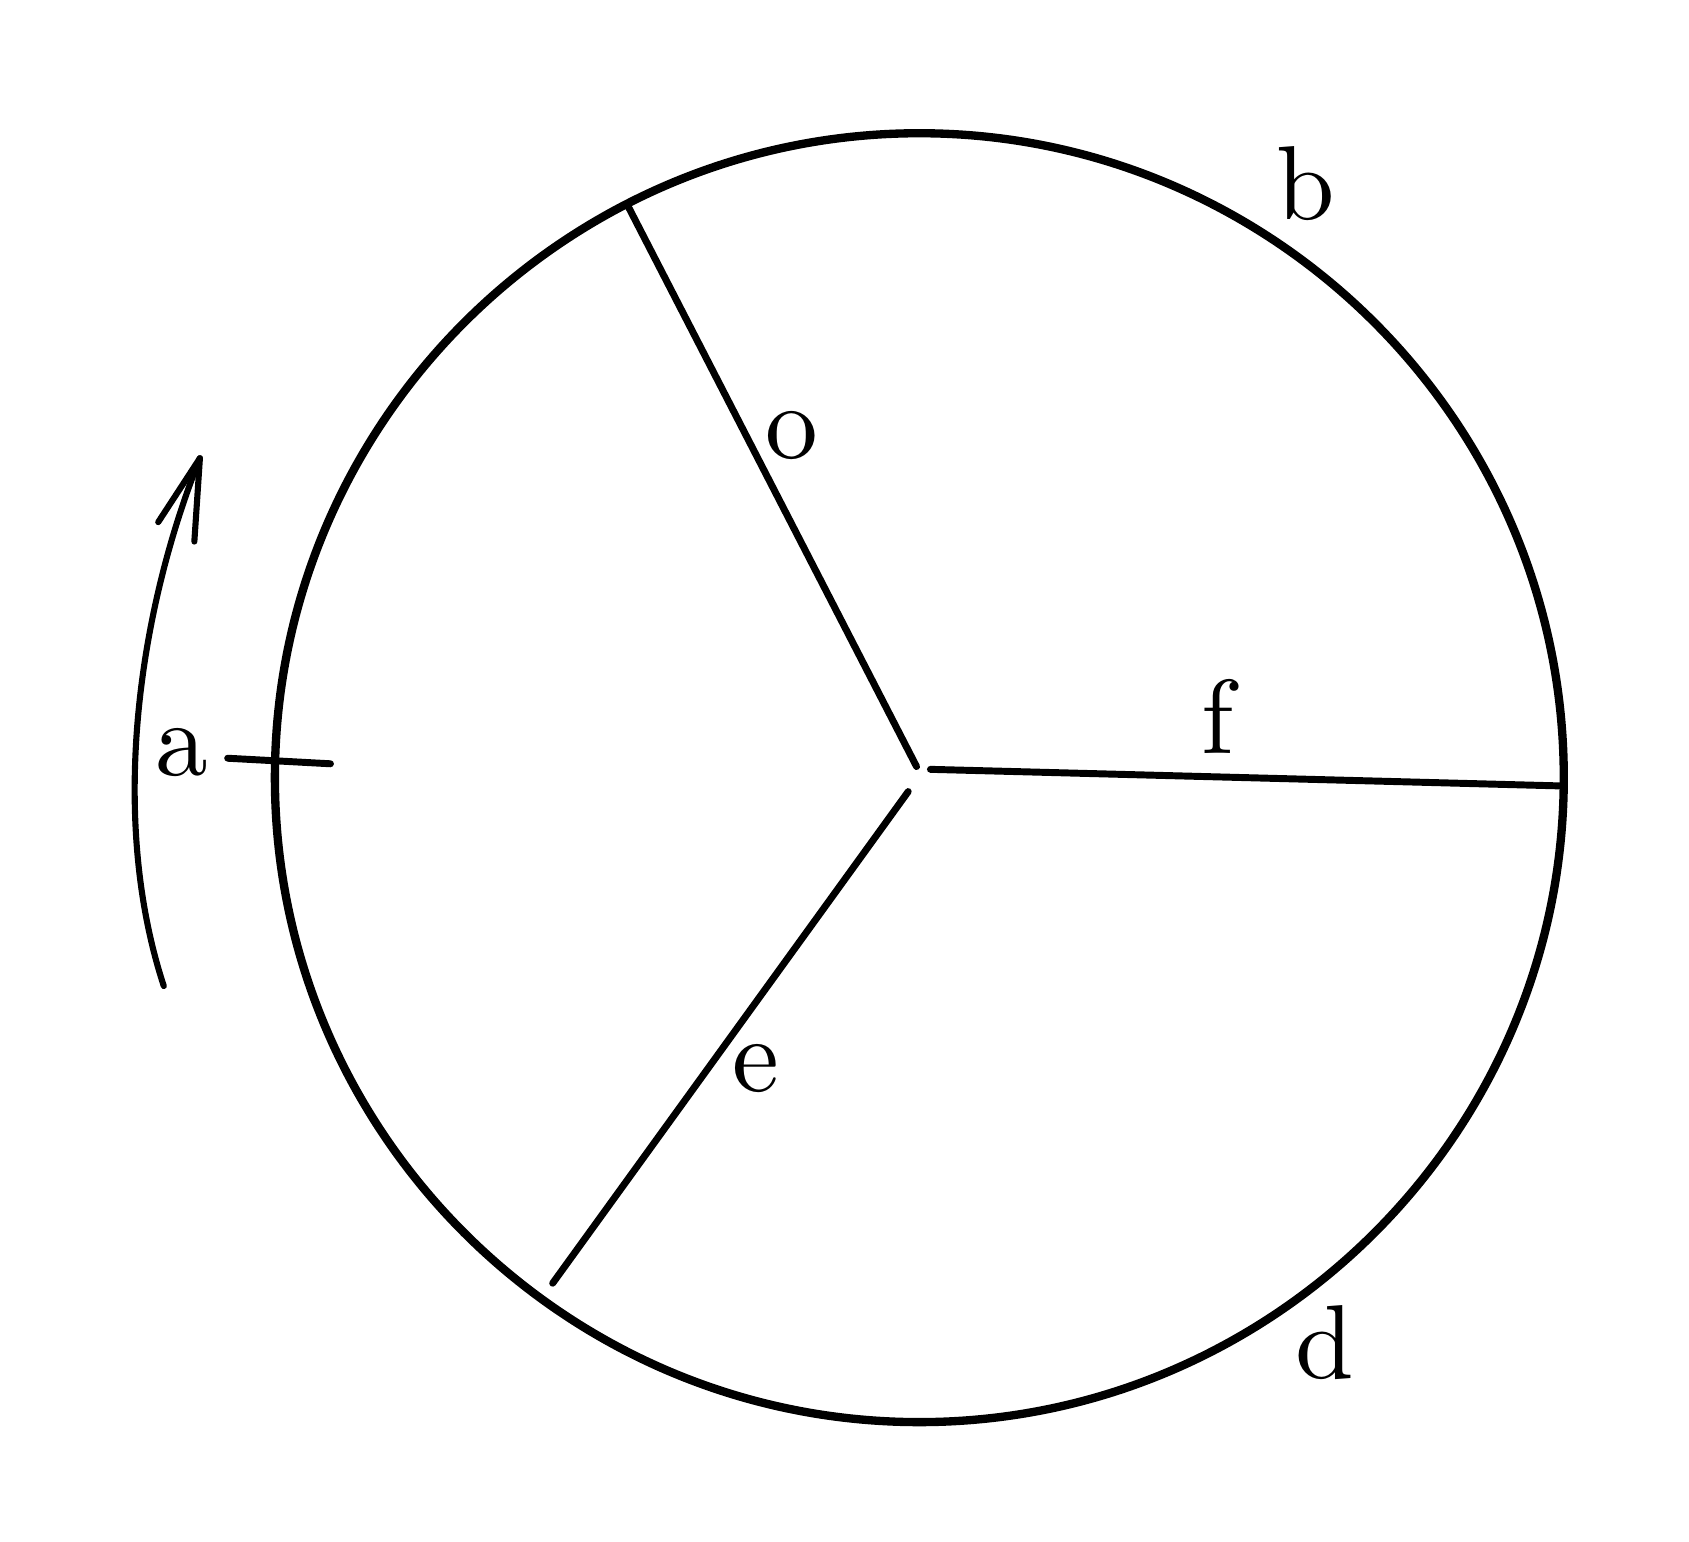
\begin{tikzpicture}[x=1bp,y=-1bp,line cap=round,line join=round]
\path[use as bounding box] (0,0) rectangle (588,535);
\begin{pgfinterruptboundingbox}
\draw[line width=3bp] (321,38) .. controls (448.60,38) and (553,142.40) .. (553,270) .. controls (553,397.60) and (448.60,502) .. (321,502) .. controls (193.40,502) and (89,397.60) .. (89,270) .. controls (89,142.40) and (193.40,38) .. (321,38);
\draw[line width=2.5bp] (216,64) -- (320,266);
\draw[line width=2.5bp] (325,267) -- (553,273);
\draw[line width=2.5bp] (317,275) -- (189,452);
\draw[line width=2.5bp] (72,263) -- (109,265);
\draw[line width=2.2bp] (49,345) .. controls (29,284) and (40,210) .. (62,155);
\draw[line width=2.2bp] (47,178) -- (62,155) -- (60,185);
\node[inner sep=0pt,outer sep=0pt] at (55,261) {\scalebox{3.8}{\ensuremath{\mathrm{a}}}};
\node[inner sep=0pt,outer sep=0pt] at (460,56) {\scalebox{3.8}{\ensuremath{\mathrm{b}}}};
\node[inner sep=0pt,outer sep=0pt] at (275,147) {\scalebox{3.8}{\ensuremath{\mathrm{o}}}};
\node[inner sep=0pt,outer sep=0pt] at (467,473) {\scalebox{3.8}{\ensuremath{\mathrm{d}}}};
\node[inner sep=0pt,outer sep=0pt] at (262,375) {\scalebox{3.8}{\ensuremath{\mathrm{e}}}};
\node[inner sep=0pt,outer sep=0pt] at (430,248) {\scalebox{3.8}{\ensuremath{\mathrm{f}}}};
\end{pgfinterruptboundingbox}
\end{tikzpicture}
